\documentclass[conference]{IEEEtran}
\IEEEoverridecommandlockouts
% The preceding line is only needed to identify funding in the first footnote. If that is unneeded, please comment it out.
\usepackage{cite}
\usepackage{amsmath,amssymb,amsfonts}
\usepackage{algorithmic}
\usepackage{graphicx}
\usepackage{textcomp}
\usepackage{xcolor}
\usepackage{subcaption}
\usepackage{kotex}
\usepackage{multicol}
\usepackage{float}
\def\BibTeX{{\rm B\kern-.05em{\sc i\kern-.025em b}\kern-.08em
    T\kern-.1667em\lower.7ex\hbox{E}\kern-.125emX}}
\begin{document}

\title{PTSD: \textbf{P}ar\textbf{T}itioned Cache and Request \textbf{S}cheduling with \textbf{D}emand-based FTL}

\author{\IEEEauthorblockN{Junsu Im}
\IEEEauthorblockA{\textit{ICE} \\
\textit{DGIST}\\
junsu\_im@dgist.ac.kr
}
\and
\IEEEauthorblockN{Jinwook Bae}
\IEEEauthorblockA{\textit{ICE} \\
\textit{DGIST}\\
jinwook.bae@dgist.ac.kr}
}

\maketitle

\begin{abstract}
This document is a model and instructions for \LaTeX.
This and the IEEEtran.cls file define the components of your paper [title, text, heads, etc.]. *CRITICAL: Do Not Use Symbols, Special Characters, Footnotes, 
or Math in Paper Title or Abstract.
\end{abstract}

\begin{IEEEkeywords}
component, formatting, style, styling, insert
\end{IEEEkeywords}

\section{Introduction}
This document is a model and instructions for \LaTeX.
Please observe the conference page limits. 

\section{Background And Motivation}
\subsection{NAND Flash and Address Mapping}
\begin{figure}[h]
	\centering
	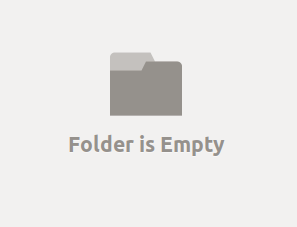
\includegraphics[width=0.2\textwidth]{image/bg.png}
	\caption{NAND Flash Chip}
	\label{fig:chips}
\end{figure}
NAND Flash의 물리적 구조는 Fig~\ref{fig:chips}과 같이 나타나 있다. NAND 칩들이 레이드 0와 비슷한 형태로 버스에 묶여져 있으며 각각의 버스는 동시에 data를 전송할 수 있는 병렬 단위가 된다. 또한 버스의 data 전송 시간 보다 칩 하나의 처리시간이 더 오래걸리기 때문에 버스에 붙여진 여러개의 칩도 병렬 단위가 된다. NAND 칩은 그 물리적 특성으로 In-place Update가 지원되지 않는다. 추가적으로 읽기와 쓰기의 단위는 하나의 물리적 페이지 단위로 이루어 질 수 있지만, 삭제 연산은 페이지의 집합인 블록 단위로 이루어진다. 이러한 두가지 기기의 특성 때문에 유저의 요청을 처리하기 위해 논리적 주소와 물리적 주소의 사상이 필요하다. \par
\begin{figure}[h]
	\centering
	\begin{subfigure}[b]{0.2\textwidth}	
		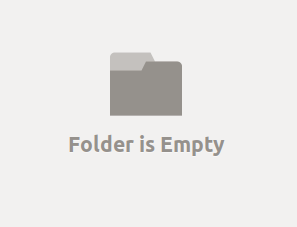
\includegraphics[width=\linewidth]{image/bg.png}
		\caption{Read/Write} \label{fig:PM}
	\end{subfigure}
	\begin{subfigure}[b]{0.2\textwidth}	
		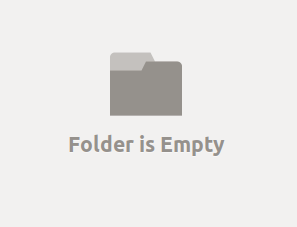
\includegraphics[width=\linewidth]{image/bg.png}
		\caption{Garbage Collection} \label{fig:GC}
	\end{subfigure}
	\caption{Page Mapping}
\end{figure}
일반적으로 성능상의 문제로 인해 사상 정보 전체를 DRAM에 저장해 두는 Page Mapping 기법을 사용한다.
DRAM 내부에는 LBA-PPA 쌍의 table이 존재하고 사용자의 요청은 이러한 사상 정보를 참고해 처리하게 된다.
PPA는 LBA와 독립적으로 존재하기 때문에 LBA에 특정한 PPA에 할당할 수 있으며 NAND Flash는 이러한 특징을 이용해 Fig~\ref{fig:chips}에서의 병렬 유닛에 맞추어 PPA를 할당하게 된다.\par
Fig~\ref{fig:PM}은 Page Mapping에서의 읽기/쓰기의 흐름을 보여준다. 들어오는 쓰기 요청은 물리적 공간에서 Logging의 형태로 적히게 되며 존재하던 정보가 새로이 들어오게 될 때 기존의 물리적 페이지가 더 이상 쓰이지 않는다는 Invalid 표시를 해두고 나중에 Garbage Collection(GC)를 통해 해당 영역을 다시 쓰게끔 동작한다.

\subsection{Garbage Collection(GC)}
GC는 더 이상 유저 쓰기 요청을 처리할 수 없을 때 발생한다. GC의 동작은 NAND의 지우기 단위인 블록의 크기로 진행되며 세가지 단계로 나누어 진다. 첫 번째로 어떠한 블록을 GC할 것인가에 대한 대상 선택의 단계이다. 이 단계에서는 Invalid 페이지가 많은 블록을 고르거나 워크로드에 맞게 Cost-benefit을 계산해 처리하는 방식이 있다. 본 논문에서는 전자의 방법을 사용하고 있다. 두 번째 단계로 Valid 페이지를 다른 블록에 Copy하는 작업이며 마지막으로는 해당 블록을 지우는 연산으로 마무리 된다.
쓰기, 읽기 연산보다 지우는 연산이 열 배 이상 걸리며 GC도중 Copy 연산이 빈번하게 일어나기 때문에 NAND 성능의 병목이 GC에서 주로 나타난다. 때문에 GC의 부하를 줄이기 위해 물리적 공간보다 적은 영역을 호스트에게 노출해 Invalid를 더 많이 분포하게 하는 over provisioning영역이 존재한다. 기본적으로 이 영역의 비율은 물리적 공간의 7\%에서 50\%까지 두게 된다.

\subsection{FTLs on limited memory environment}
\begin{figure}[h]
	\centering
	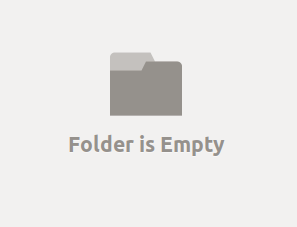
\includegraphics[width=0.2\textwidth]{image/bg.png}
	\caption{Variable Mapping Method in limited DRAM}
	\label{fig:Map}
\end{figure}
앞서 언급했듯이 본 논문은 DRAM이 제한된 환경에서의 연구를 목적으로 하고 있다. 이때까지 제시된 논문은 Fig~\ref{fig:Map}와 같이 많은 문제점이 존재한다. 블록 단위의 사상과 Hybrid사상은 읽기 연산의 경우 한 번에 접근이 가능하지만 GC연산이 빈번하게 호출되기 때문에 쓰기 연산이 많이 발생하게 되고 쓰기연산은 NAND의 수명을 줄일 뿐 아니라 많은 시간이 소모 되기 때문에 사용하기 어렵다. 반면 Demand Based사상의 경우 합리적인 읽기 쓰기 비용을 가지고 있지만 Cache의 Dirty가 eviction 문제로 인해 읽기 연산의 시간을 예상하기 힘들다. PTSD는 Demand Based 사상을 기반을 하여 해당 사상의 문제점을 분석해 새로운 방법을 제시한다.

\subsection{Demnad based FTL}

\section{PTSD}
\begin{figure}[h]
	\centering
	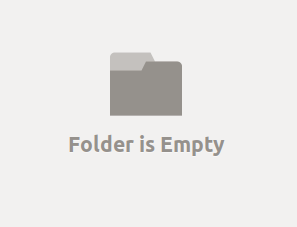
\includegraphics[width=0.3\textwidth]{image/bg.png}
	\caption{PTSD platform}
	\label{fig:PTSD}
\end{figure}
Fig~\ref{fig:PTSD}는 본 연구에서 제작된 PTSD에 대한 그림이다. PTSD는 크게 세가지 부분으로 나뉘며 위쪽의 유저의 요청을 처리하는 Interface 계층과 실제적인 알고리즘이 동작하는 Algorithm계층, 마지막으로 NAND와 직접 적으로 통신하는 Device 계층이 있다. Interface에는 유저의 요청을 보관하는 큐가 존재하며 이 큐에서 요청들을 가져와 Alogrithm 계층으로 보내준다. Alogorithm 계층을 지난 요청들은 PPA를 할당 받게 되고 Device 계층을 통해 NAND에 접근하게 된다.
\subsection{Cache Partitioning}
\begin{figure}[h]
	\centering
	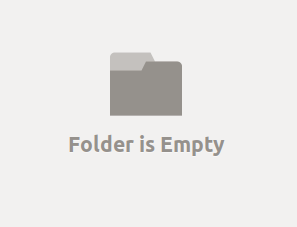
\includegraphics[width=0.3\textwidth]{image/bg.png}
	\caption{Cache partition}
	\label{fig:cache}
\end{figure}
Motivation 섹션에서 보았듯이 Demand-based FTL에서 읽기 요청을 보장하지 못하는 것은 Cache 공간이 부족한 상황에서 Dirty eviction이 발생해 읽기를 수행함에도 불구하고 쓰기 연산이 발생하기 때문이다. 이러한 문제점을 해결하기위해 Cache Partition 기법을 제안한다. 이는 Fig~\ref{fig:cache}와 같이 페이지 단위의 CMT 구조를 기반으로 고안되었다. SSD 내부 메모리에서 CMT로 사용되는 영역을 논리적으로 나누어, clean 영역에서는 clean 상태의 사상 페이지만, dirty 영역에서는 dirty 상태의 사상페이지만 저장한다. 그리고 저장된 사상 페이지들은 각 영영게서 LRU 교체 정책을 통해 관리된다.\par
\begin{itemize}
	\item{읽기 요청}\\
	읽기 요청이 SSD로 들어오면 먼저 Cache를 살펴본다. 관련된 사상 페이지가 dirty 영역에 저장되어 있더라도 참조는 가능하다. cache 참조를 통해 주소 변환관계를 알 수 있다면, 해당 물리 주소에 저장된 데이터를 읽는단. 하지만 cache miss가 발생할 경우, 즉 clean, dirty 영역 모두에서 참조를 실패했다면 clean 영역 내의 LRU 알고리즘을 통해 참조된 지 가장 오래된 클린 페이지를 쫓아낸다. 이렇게 하면 읽기 요청 중에 추가적인 쓰기 작업이 발생하지 않는 것을 쉽게 보장할 수 있다. 따라서 해당 기법을 사용할 때, 읽기 요청은 최악의 경우 cache miss로 인한 사상 페이지 읽기와 데이터 읽기로 총 2번의 읽기로 완료된다.
	\item{쓰기 요청}\\
	반면에 쓰기 요청 중에는 dirty 영역에서 페이지를 비워주게 되기 때문에, 캐시 적중에 실패할 경우 사상 페이지의 쓰기가 항상 동반하게 된다. 이는 기존 Demadn-based FTL에서 읽기 요청 중에 발생하던 추가 쓰기 작업들을, 쓰기 요청 중에 발생하도록 미룬 것과 같다. 그리고 cache에서 참조에 성공하는 경우, 두 가지 상황이 발생한다.\par
	먼저 dirty 영역세어 적중된 경우 새롬게 쓰이는 물리 주소로 엔트리를 갱신한다. dirty 영역에서 존재하는 사상 페이자들은 모두 dirty 상태이기 때문에 이 작업 중에 사상 페이지의 상태 변화는 없다. 그리고 해당 페이지를 dirty 영역에서 자체적으로 관리하는 LRU 알고리즘에서 갱신해 준다.\par
	반면에 이미 clean 영역으로 올라온 사상 페이지에서 cache 적중이 될 경우에는 추가적인 연산이 발생한다. 쓰기 요처이이 발생하면 주소 변환 테이블의 엔트리도 함께 갱신되기 때문에, 쓰기 요청에 한 번이라도 적중된 사상 페이지는 dirty 상태로 전환되어 버린다. 그러므로 해당 페이지는 더 이상 clean 영역에 머무를 수 없게 된다. 이 때 cache 영역을 제한하지 않고 단순히 dirty 영역으로 이전시키는 것은, 모든 cache 영역이 dirty 상태의 사상 페이지로 채워질 수 있기 때문에 문제가 된다. 이 경우 다음에 들어오는 읽기 요청에서 cache 적중에 실패하면 쓰기 작업이 수행되고 곧바로 응답시간에 영향을 미치게 된다. 이는 곧 clean 영역의 공간을 어느 정도 보장해야 한다는 것을 의미한다. 그래서 우리는 clean 영역에서 dirty 영역으로 이전될 때, dirty 영역이 가득 차 있다면 해당 cache 영역의 희생 페이지를 SSD에 써서 각 영역의 공간을 확보하게끔 하였다.\par
	각 영역의 크기는 읽거나 쓰기 목적에 따라 다르게 설정할 수 있지만 본 논문에서는 50:50의 비율로 설정하여 기법의 효과를 실험하였다.
\end{itemize}
\subsection{I/O Scheduling}
cache partition 기법을 적용한다고 하여도 문제점이 한가지 존재한다. 그것은 바로 쓰기 연산이 비동기적으로 이루어진다는 것이다. 유저의 쓰기 요청은 병렬 유닛을 전부 활용하기 위해 최대한 비동기 연산으로 처리를 하게 된다. 또한 병렬 연산을 최대한 활용하기 위해 Fig~\ref{fig:PTSD}의 그림처럼 Buffer가 존재하게 된다. Buffer가 가득 차 있지 않다면 요청이 금방 끝나지만 Buffer가 가득 차게 된다면 Buffer를 flush 해준다. 해당 쓰기 요청은 Buffer를 flush를 하라는 명령만을 내릴 뿐 해당 연산이 끝날 때 까지 대기하지 않기 때문에 바로 다음 연산이 읽기일 경우 해당 flush 연산의 시간이 읽기 연산으로 부하가 넘어가게 된다.\par
이 문제를 해결하기 위해 Interface 계층의 큐를 이용하였다. Interface의 큐 내부의 요청들 중 읽기와 쓰기 요청을 구분한다. 어느 순간 Buffer가 가득차게 될 경우 flush를 해야될 시점이 오면 flush를 하지 않고 write\_stop flag를 set 한다. 해당 flag가 설정이 되어 있을 경우 Interface의 큐 중 읽기 요청만을 처리를 우선적으로 진행한다. 그 뒤 큐 내부의 요청이 모두 쓰기 요청으로 가득 차게 됬을 때 flush를 진행하고 해당 마지막 쓰기 요청은 동기 방식으로 처리해 최대한 읽기 요청의 응답 시간을 보호하도록 scheduling을 진행한다.\par
\subsection{Write Optimization}
\begin{figure}[hbt]
	\centering
	\begin{subfigure}[b]{0.3\textwidth}	
		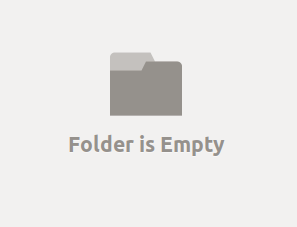
\includegraphics[width=\linewidth]{image/bg.png}
		\caption{Different cache layout} \label{fig:Dcache}
	\end{subfigure}
	\begin{subfigure}[b]{0.3\textwidth}	
		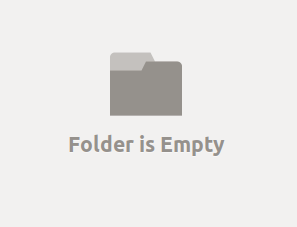
\includegraphics[width=\linewidth]{image/bg.png}
		\caption{Batch update} \label{fig:batch}
	\end{subfigure}
\end{figure}
~\ref{fig:cache}처럼 페이지 단위로 CMT를 구성하면, 임의 트래픽의 워크로드에서 부가적인 쓰기 연산이 많아지고 쓰기 성능이 저하되는 문제가 발생한다. 이는 추후에 평가에서도 볼 수 있듯 demand-based FTL은 물론이고, cache partition 상황에서 더 뚜렷하게 나타난다. 때문에 우리는 기존의 cache partion기법에서 dirty 영역을 엔트리 단위로 이어 쓰도록 하여 쓰기 성능을 최적화 하였다. 읽기 요청은 기존 구조와 같기 때문에 이전 흐름을 그대로 따라가지만, 쓰기 요청은 동작 방식이 바뀌게 된다.
\begin{itemize}
	\item{쓰기 요청}\\
	쓰기 요청은 발생할 때마다 CMT의 엔트리를 갱신해야 한다. 페이지 단위 저장 방식에서는 한 엔트리를 갱신하기 위해 전체 사상 페이지를 함께 메모리에 올려야했다. 이는 임의 트래픽의 쓰기 워크로드에서 매우 비효율적으로 동작한다. 반면 쓰기 요청에서 갱신하는 엔트리는 사상 페이지를 메모리에 올리지 않아도 변경 사항을 기록할 수 있다. Fig~\ref{fig:Dcache}와 같이 dirty 영역에 엔트리 단위로 이어쓰게 되면 불필요한 쓰기 작업을 없앨 수 있다. 
	\item{Batch-update}\\
	부족한 메모리를 위해 엔트리를 비워야하는 상황이 되면, 엔트리 단위 저장 방식에서 batch-update 를 통해 희생 엔트리와 같은 사상 페이지의 엔트리들을 함께 써야 한다. 만약 희생 엔트리 1개만 SSD에 써줄 경우 부가적인 쓰기 연산이 매우 빈번하게 발생하기 때문이다. 본 기법에서는 Fig~\ref{fig:batch}와 같이 dirty 영역의 엔트리들을 사상페이지 별로 관리하고 쫓아내는 상황이 되면 희생페이지를 정해서 batch-update하였다.\par
	이 경우 희생 페이지를 정하는 데이 있어 다양한 교체 정책이 사용될 수 있다. 예를 들어, 페이지 단위로 LRU 알고리즘을 사용하거나, dirty 상태의 엔트리가 가장 많은 페이지를 선택하는 greedy 알고리즘을 사용할 수 있다. 본 논문에서는 greedy 알고리즘 방식을 채택하여, batch-update 효과를 최대한 활용하였다.
\end{itemize}
\subsection{Future Work}
언급한 세가지 최적화를 통해 많은 부분을 개선할 수 있었지만, 해당 기법을 통해 다양한 이슈들이 발생하는데 본 연구에서 시간상의 이유로 해결하지 못하였다. 이는 남은 작업으로 남겨 두어 추후 연구를 진행할 계획이다. 
\begin{itemize}
	\item{Limitaion of I/O scheduling}\par
	현재 적용한 I/O scheduling은 유저의 요청을 잠시간 받지 않게 하여 장치의 응답시간을 높이는 방식이다. 이러한 방식은 결과적으로 전체적인 요청에 대해 최적화가 진행되지 않았다고 볼수 있다. 그렇기 때문에 추후 연구에서는 이러한 문제점을 개선 하여 유저의 요청을 지속적으로 처리할 수 있는 Scheduling 알고리즘의 개발이 필요하다. 또한 현재의 NAND 칩에서 쓰기 발생시 읽기 요청이 들어올 때 읽기 요청을 선점하여 처리할 수 있는 하드웨어도 개발 되고 있다. 해당 하드웨어를 사용할 경우 위의 문제를 쉽게 해결할 수 있을것이라 기대된다.
	\item{Adaptive partioning}\\
	본 논문에서 clean, dirty cache의 영역이 50:50의 비율을 유지하고 있다. 하지만 이는 워크로드의 특성을 제대로 활용하지 못할 수 있다. 읽기가 많은 요청에서는 clean cache의 영역이 더 많은 비율을 차지할 시 성능이 더 좋아질 것이며 반대의 경우 또한 마찬가지이다. 즉, 워크로드를 모니터링을 진행한 다음 PID 컨트롤과 같은 방식을 이용한다면 조금 더 최적화된 기법을 적용할 수 있을 것이다.
\end{itemize}
\section{Evaluation}
\begin{figure}[h]
	\centering
	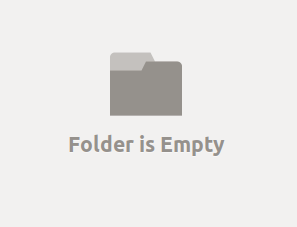
\includegraphics[width=0.3\textwidth]{image/bg.png}
	\caption{임베디드 보드}
	\label{fig:zync}
\end{figure}
PTSD의 기법의 효과를 증명하기 위해 우리는 PTSD(PART), Demand-base FTL(DFTL), Page FTL(OPT)의 알고리즘을 실제 시스템과 유사한 임베디드 보드(Fig~\ref{fig:zync})에서 진행하였다.
\subsection{Setting}
실험의 설정은 모두 임베디드 보드에서 진행되었으며 해당 보드의 스펙은 Fig~\ref{fig:zync}에 나와 있다. 실험은 소프트웨어 적으로 해당 SSD의 총 용량을 16GB로 설정하여 진행 하였으며 over provisioning 영역은 20\%를 두었다. PTSD와 DFTL은 전체 OPT의 메모리의 20\%가 있다는 가정으로 모든 실험을 진행 하였다. 실험은 총 32GB의 임의 쓰기후 임의 읽기를 진행하였다. 큐 뎁스는 128로 설정하였다.
\subsection{Read CDF Trend}
\begin{figure}[h]
	\centering
	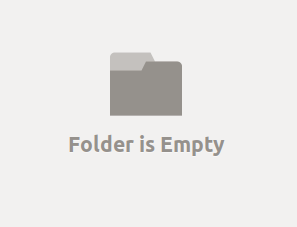
\includegraphics[width=0.3\textwidth]{image/bg.png}
	\caption{cdf 결과}
	\label{fig:cdf1}
\end{figure}
Fig~\ref{fig:cdf1}은 cache partition의 효과를 보이기 위해 진행한 실험이다. 기존의 DFTL에 비해서 평균적인 성능이 상당히 많은 부분 앞당겨 진것을 알 수 있다. 90\%지점 까지, 거의 모든 요청들이 OPT에 비해서 1번의 읽기가 추가되는 모습을 보이고 있다. 다만 스펙에서 나온것 처럼 140micro sec이 차이가 나는 것은 아닌데 이 원인은 큐 뎁스가 128이기 때문에 큐 대기시간이 각각의 요청에서 추가되었기 때문이다. \par
평균적인 성능은 개선된것을 확인할 수 있었으나 중요한 꼬리 응답시간에서는 거의 효과가 없다는 것을 알 수 있다. 원인은 PTSD 섹션에서 설명한 비동기 쓰기 연산으로 인한 것이다.\par
\begin{figure}[hbt]
	\centering
	\begin{subfigure}[b]{0.2\textwidth}	
		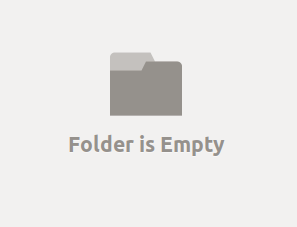
\includegraphics[width=\linewidth]{image/bg.png}
		\caption{cdf} \label{fig:cdf2}
	\end{subfigure}
	\begin{subfigure}[b]{0.2\textwidth}	
		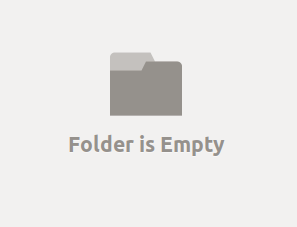
\includegraphics[width=\linewidth]{image/bg.png}
		\caption{zoom in} \label{fig:cdf2_zoom}
	\end{subfigure}
	\caption{PTSD scheduling cdf}
\end{figure}
Fig~\ref{fig:cdf2}와 Fig~\ref{fig:cdf2_zoom}은 scheduling알고리즘을 추가한 결과를 보여준다.Fig~\ref{fig:cdf2}의 경우를 보았을 때 scheduling이 추가 했을 때 평균적인 성능이 약간 좋아진것을 알 수 있다. 또한 Fig~\ref{fig:cdf2_zoom}의 경우Fig~\ref{fig:cdf2}의 결과에서 꼬리 응답 시간의 결과를 보기 위해 80\% 지점에서 부터 다시 CDF를 그린것이다. 해당 그림으로 인해 꼬르 응답 시간의 경우 확연한 성능의 차이가 있다는 것을 알수 있다.
\subsection{Read distribution}
\begin{figure}[h]
	\centering
	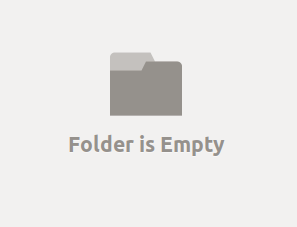
\includegraphics[width=0.3\textwidth]{image/bg.png}
	\caption{읽기요청의  응답 시간 분포}
	\label{fig:dist}
\end{figure}
CDF의 형태가 아닌 각각의 응답 시간의 분포도를 찍어서 보았다. 해당 그래프를 통해 이번 연구의 큰 목표였단 읽기 응답시간의 분포를 앞으로 당기는 것을 확연히 보여줄 수 있었다.
\subsection{Write performance}
\begin{figure}[h]
	\centering
	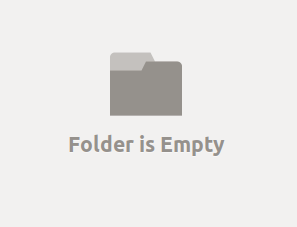
\includegraphics[width=0.3\textwidth]{image/bg.png}
	\caption{총 성능}
	\label{fig:through}
\end{figure}
쓰기 성능의 개선 효과를 보기 위해 총 성능 또한 각 알고리즘 별로 찍어 보았다. PART에 비해  PART-SCHED의 경우 약간 성능이 하락 하는 것을 보였는데 해당 원인이 scheduling으로 인한 성능 저하로 보인다. WRITEOPT의 경우 OPT를 제외한 모든 곳보다 성능상 우위에 있다는 것을 알 수 있는데 엔트리 단위의 CMT 관리가 효율적이라는 것을 보인다. 해당 결과는 PART-SCHED에 비해 약 10\%가량 개선이 있음을 알 수 있다. OPT를 제외한 전체적인 성능이 크게 차이가 없는 이유는 GC의 부하가 크기 때문이다. 모든 알고리즘은 GC에서 같은 로직으로 수행되기 때문에 GC 부하가 많은 시간을 차지할 때 비슷한 성능을 보인다. 

\section{Conclusion}
본 논문에서는 Demand-base FTL의 늘어지는 읽기 응답 시간을 줄이기 위해 cache를 두 영역으로 나누어 읽기 응답시간을 보장하는 cache 분리 기법을 소개했다. \par
제안된 기법은 Demand-base FTL의 읽기 응답시간이 느려지는 원인 분석을 바탕으로, 일기 요청 중 방해 받을 수 있는 요소들을 없앴다. 그리고 요구 기반 FTL의 두 가지 테이블 구성 빙식의 장점을 함께 취하여 쓰기 성능 또한 최적화시켰다. 그리고 임베디드 보드에서 FTL의 성능을 측정하여 임의 쓰기와 읽기 실험에비해 1.15배 성능이 개선됨을 보였다.\par
이후 연구에서는 scheduling 기법의 변화와 워크로드 특성을 반영한 partition기법을 통해 PTSD가 더 잘 동작하도록 수정할 예정이다.

\end{document}
